\par
Notre application repose sur une architecture 3-Tiers\footnote{L'architecture trois tiers, aussi appelée architecture à trois niveaux ou architecture à trois couches, est l'application du modèle plus général qu'est le multi-tier. L'architecture logique du système est divisée en trois niveaux ou couches : couche de présentations, couche de traitement, couche d'accès aux données. C'est une architecture basée sur l'environnement client-serveur. Wikipédia.}\\

Cette architecture nous permet de mieux distinguer chaque partie, d'où une conception plus optimale. Ainsi, nous aurons trois parties distinctes : 

\begin{itemize}

	\item couche client (les joueurs) : cette partie regroupe les joueurs qui se connectent au serveur. Nous aurons une abstraction des joueurs physiques, une représentation des joueurs en mémoire du côté de la couche client. Ci dessous le diagramme de classe de la couche client :

\begin{figure}[!h]
	\centering
	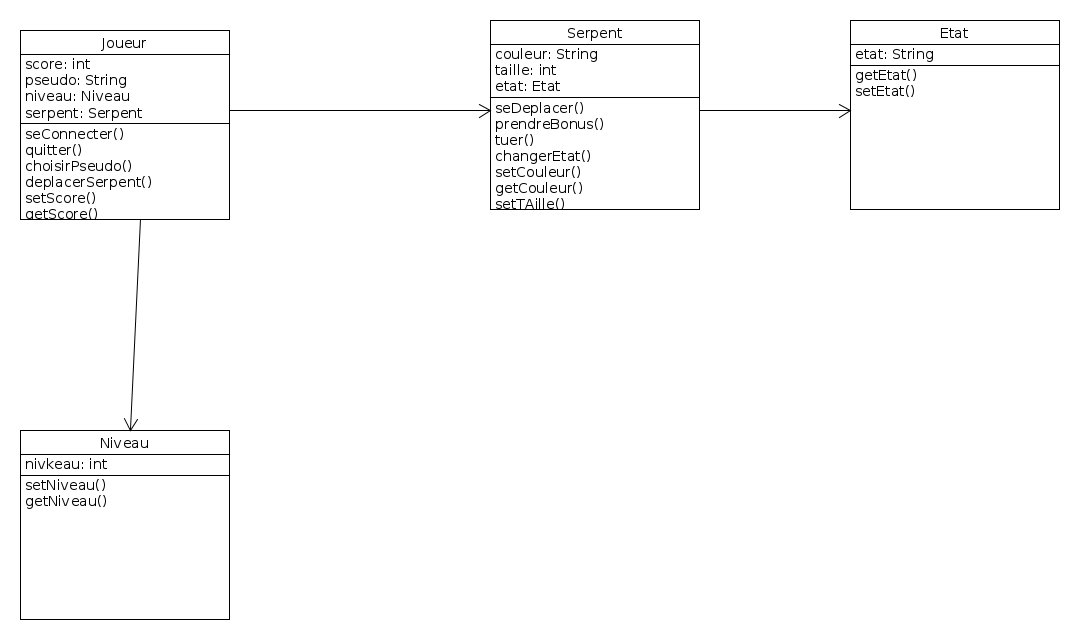
\includegraphics[scale = 0.40]{img/diagClient.png}
	\caption{Diagramme de classe de la couche client}
\end{figure}

	
	\item couche serveur : cette partie regroupe à la fois le serveur, la vue, le modèle (les classes métiers). \\
	Le serveur assure tout ce qui est communication avec les joueurs, centralise leurs actions. Le modèle est une abstraction des joueurs physiques, une représentation des joueurs en mémoire du côté dans la couche serveur. La vue représente le plan, la partie visible qui sera partagée par tous les joueurs, la partie qui permet aux joueurs d'interagir avec le jeu, serveur. \\
	
	Afin de mieux séparer les composants de cette couche, nous structurons cette couche en utilisant le patter MVC, ainsi nous aurons de manière distincte le serveur qui est en même temps le contrôleur, la vue et le modèle. Ci dessous une représentation du pattern MVC :

\begin{figure}[!h]
	\centering
	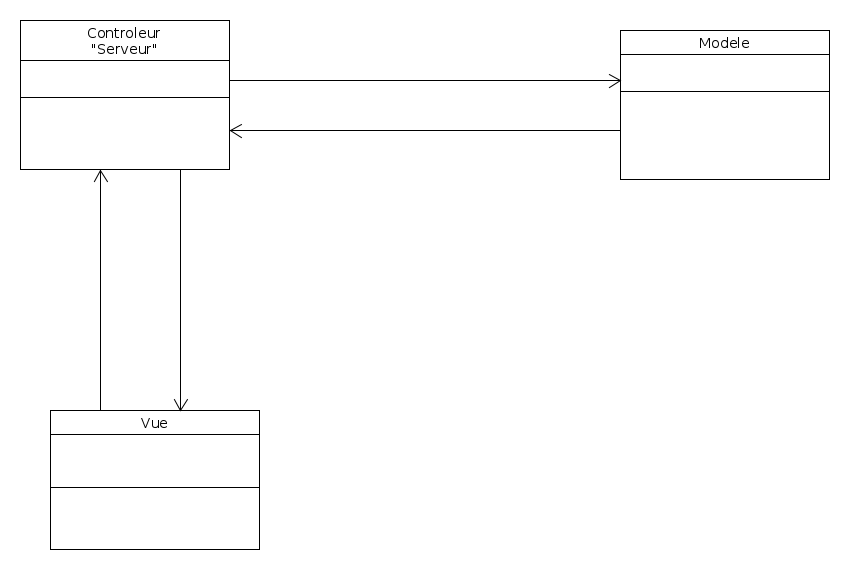
\includegraphics[scale = 0.40]{img/diagMVC.png}
	\caption{Représentation du design pattern MVC}
\end{figure}

	
	Le serveur communique avec la vue et le modèle via le pattern Façade. Ci dessus, le diagramme des classe du pattern MVC intégrant le pattern Façade du serveur :

\begin{figure}[!h]
	\centering
	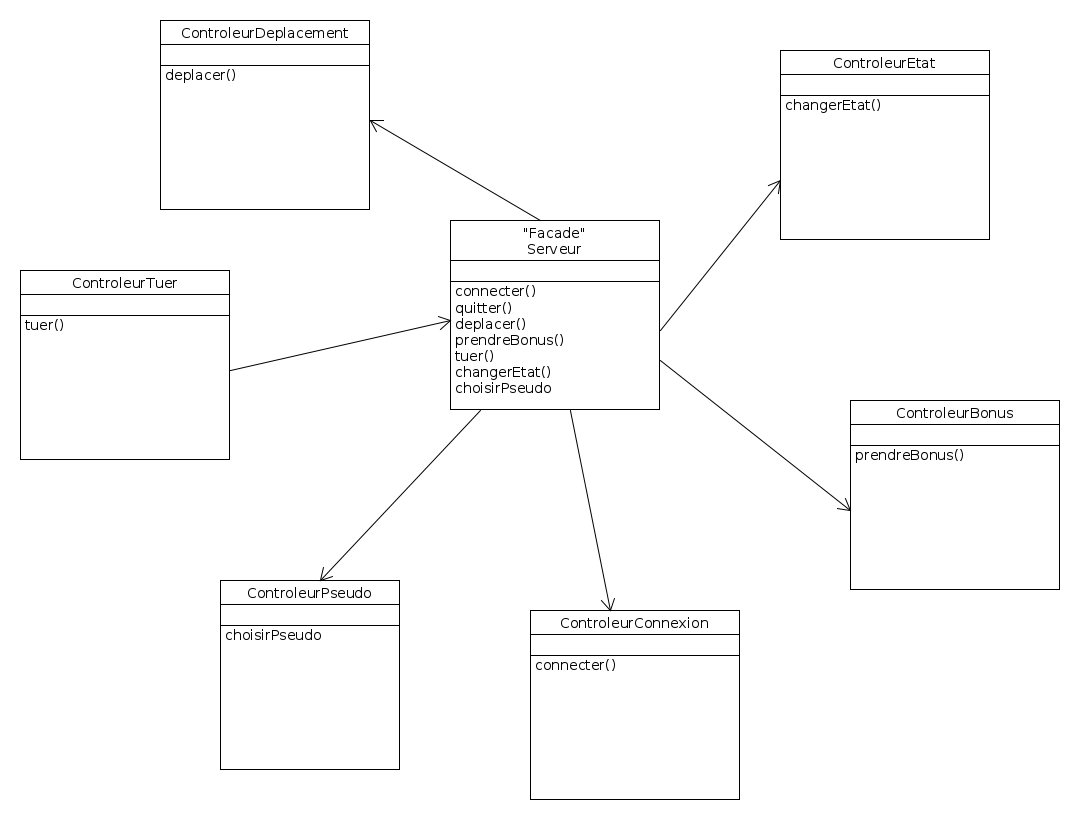
\includegraphics[scale = 0.40]{img/diagServeur.png}
	\caption{Diagramme de classe de la couche serveur}
\end{figure}
\newpage
	
	\item couche persistance : la persistance des données est gérée dans cette partie. \\
	Les données sont une abstraction des joueurs en base de données. Dans cette couche, les données sont des objets des classes métiers. \\
	
\end{itemize}

\par
Pour faire communiquer ces trois couches, nous mettons en place une conception basée sur différents designs patterns. \\

\par
La communication entre la couche client et celle serveur se fera via le pattern Proxy. Ci dessus une représentation de la communication les couches client et serveur :
\begin{figure}[!h]
	\centering
	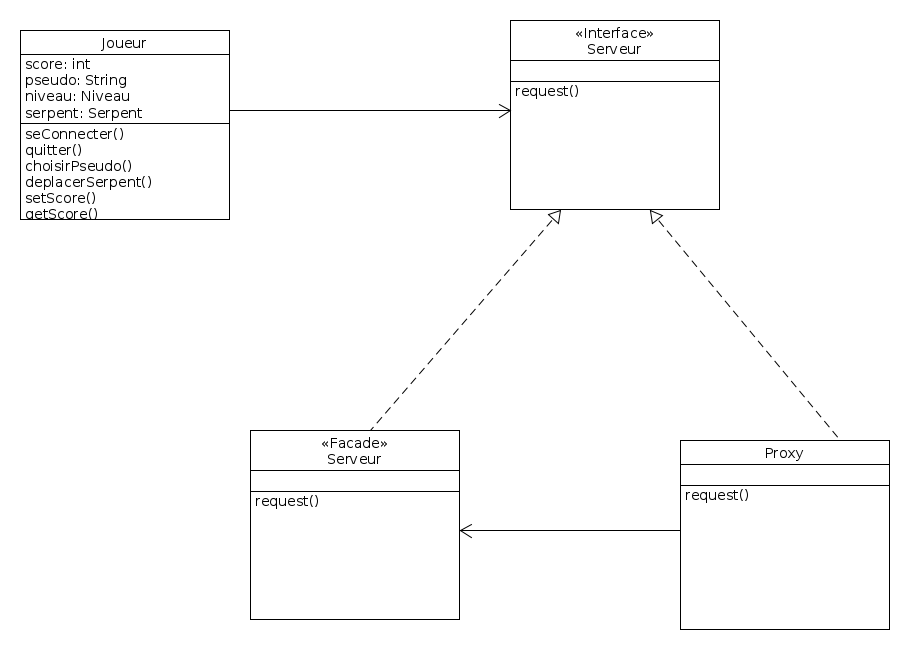
\includegraphics[scale = 0.40]{img/diagProxy.png}
	\caption{Diagramme de classe du pattern Proxy}
\end{figure}
\newpage

\par
La persistance des données passe par le pattern DAO. Ci dessous une représentation de la persistance des données :
\begin{figure}[!h]
	\centering
	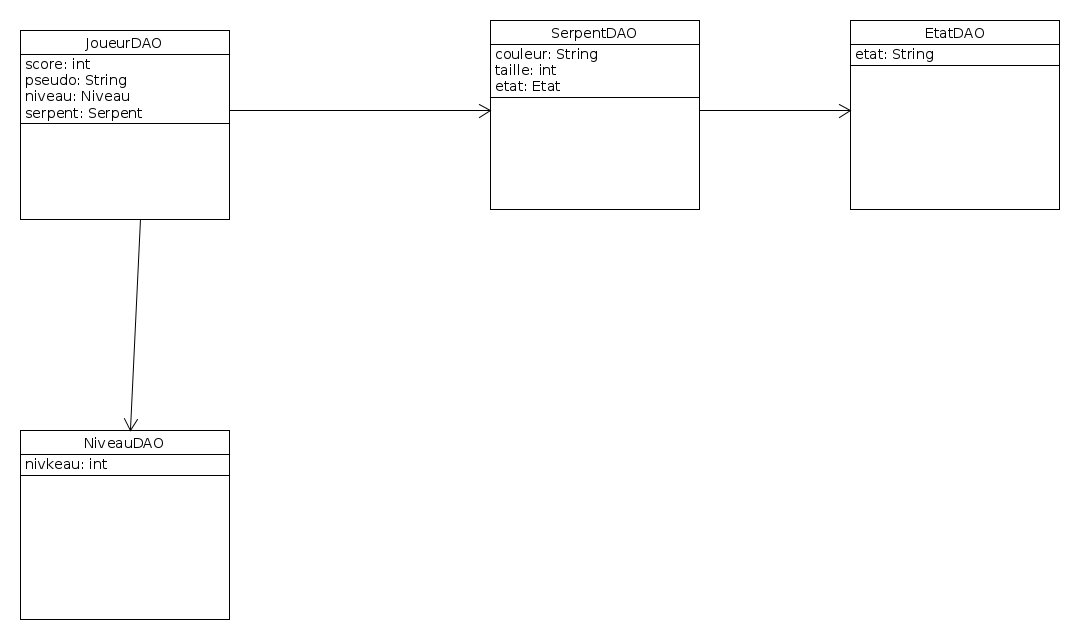
\includegraphics[scale = 0.40]{img/diagDAO.png}
	\caption{Diagramme de classe du pattern DAO}
\end{figure}


